%%%%%%%%%%%%%%%%%%%%%%%%%%%%%%%%%%%%%%%%%%%%%%%%%%%%%%%%%%%%%%%%%%%%%%%%%%%%%%%%%%%%%%%%%%%%%%%
%%%%%%%%%%%%%%%%%%%%%%%%%%%%%%%%%%%%%%%%%%%%%%%%%%%%%%%%%%%%%%%%%%%%%%%%%%%%%%%%%%%%%%%%%%%%%%%
%% LaTeX-Beamer template for KIT design
%% by Erik Burger, Christian Hammer
%% title picture by Klaus Krogmann
%%
%% version 2.1
%%
%% mostly compatible to KIT corporate design v2.0
%% http://intranet.kit.edu/gestaltungsrichtlinien.php
%%
%% Problems, bugs and comments to
%% burger@kit.edu
%%
%%
%% Modified: 30.1.2013, Schwall

\documentclass[12pt]{beamer}

%% SLIDE FORMAT
\usepackage{templates/beamerthemekit}

%% german time format (e.g 30.1.2013)
\usepackage{datetime}
\usepackage{bbm} %% Used to denote the indicator function
%\usepackage[T1]{fontenc}
%\usepackage{amssymb}
\usepackage{amsmath}
\usepackage{graphicx}
\usepackage{color,psfrag}
\usepackage{subfig}

\newdateformat{germandate}{\THEDAY.\THEMONTH.\THEYEAR}
\newdateformat{americandate}{\THEMONTH/\THEDAY/\THEYEAR}

% use these packages for PCM symbols and UML classes
\usepackage{templates/tikzkit}
\usepackage{templates/tikzuml}
\usepackage{siunitx}

\usepackage{times}
\usepackage{tikz}


\usepackage[english]{babel}
\usepackage{csquotes}
\setquotestyle{american}
\usepackage[language=american,autocite=footnote,citestyle=authortitle,citetracker=true,backend=biber,babel=other]{biblatex}
\addbibresource{../refs.bib}

\usepackage{verbatim}
\usetikzlibrary{arrows,shapes}

\setbeamerfont{footnote}{size=\tiny}
%%%%%%%%%%%%%%%%%%%%%%%%%%%%%%%%%%%%%%%%%%%%%%%%%%%%%%%%%%%%%%%%%%%%%%%%%%%%%%%%%%%%%%%%%%%%%%%
%%%%%%%%%%%%%%%%%%%%%%%%%%%%%%%%%%%%%%%%%%%%%%%%%%%%%%%%%%%%%%%%%%%%%%%%%%%%%%%%%%%%%%%%%%%%%%%
% the presentation starts here

\usepackage{datetime}
\newdate{date}{21}{09}{2016}

\usepackage[framemethod=TikZ]{mdframed} %% For inserting the individual contributions in box
\mdfdefinestyle{MyFrame}{%
    linecolor=kit-green100,
    outerlinewidth=0.8pt,
    roundcorner=8pt,
    frametitlerule=true,
    frametitlebackgroundcolor=kit-green30,
    innertopmargin=5pt,
    frametitlealignment=\center,
    %frametitleaboveskip=-5pt,
}


\newcounter{theo}[section]
\newenvironment{theo}[1][]{%
\stepcounter{theo}%
\ifstrempty{#1}%
{\mdfsetup{%
frametitle={%
\tikz[baseline=(current bounding box.east),outer sep=0pt]
\node[anchor=east,rectangle,fill=blue!20]
{\strut Theorem~\thetheo};}}
}%
{\mdfsetup{%
frametitle={%
\tikz[baseline=(current bounding box.east),outer sep=0pt]
\node[anchor=east,rectangle,fill=blue!20]
{\strut Theorem~\thetheo:~#1};}}%
}%
\mdfsetup{innertopmargin=10pt,linecolor=blue!20,%
linewidth=2pt,topline=true,
frametitleaboveskip=\dimexpr−\ht\strutbox\relax,}
\begin{mdframed}[]\relax%
}{\end{mdframed}}


\newenvironment{myenv}[1]
  {\mdfsetup{
    frametitle={\colorbox{white}{\space#1\space}},
    innertopmargin=10pt,
    frametitleaboveskip=-\ht\strutbox,
    frametitlealignment=\center
    }
  \begin{mdframed}%
  }
  {\end{mdframed}}



% english vs. ngerman
\selectlanguage{english}

\title[Performance Analysis of Interweave Cognitive Radio Systems with Imperfect Channel Knowledge]{Performance Analysis of Interweave Cognitive Radio Systems with Imperfect Channel Knowledge over Nakagami Fading Channels
 }
\subtitle{VTC 2016, Montr\'eal}

\author{A. Kaushik\inst{1}, \textbf{S.K. Sharma}\inst{2}, S. Chatzinotas\inst{2}, B. Ottersten\inst{2}, F. K. Jondral\inst{1}}
\institute{\inst{1}Communications Engineering Lab, Karlsruhe Institute of Technology (KIT), Germany,\\
\and
\inst{2}SnT - securityandtrust.lu, University of Luxembourg, Luxembourg, \\
}

%% insert date in correct format
\iflanguage{english}{
	\date{21 Sept 2016}
	}{
	\date{\germandate\today}
}

\institute{\inst{1}CEL, Karlsruhe Institute of Technology (KIT), Germany and \inst{2}SnT, University of Luxembourg, Luxembourg}


%% User dedined marcro 



\newcommand{\e}[2]{{\mathbb E}_{#1}\left[ #2 \right]}
\newcommand{\s}[2]{{\frac{1}{{#1}}\sum_{n=1}^{#1}} {#2}}
\newcommand{\q}[2]{{\mathcal Q}_{#1}\left( #2 \right)}
\newcommand{\p}{\mathbb P}
\newcommand{\sub}[1]{_{\text{#1}}}
\newcommand{\supe}[1]{^{\text{#1}}}
\newcommand{\pd}{\text{P}\sub{d}}
\newcommand{\pdac}{{\text{P}}\sub{d}\supe{}}
\newcommand{\pdoc}{{\text{P}}\sub{d}\supe{}}
\newcommand{\pfa}{\text{P}\sub{fa}}
\newcommand{\pfaac}{{\text{P}}\sub{fa}\supe{}}
\newcommand{\pfaoc}{{\text{P}}\sub{fa}\supe{}}
\newcommand{\phz}{\p(\mathcal{H}_0)}
\newcommand{\pho}{\p(\mathcal{H}_1)}
\newcommand{\pc}{\text{P}\sub{c}}
\newcommand{\pcd}{\bar{\text{P}}\sub{c}}
\newcommand{\pdd}{\bar{\text{P}}\sub{d}}

\newcommand{\prcvd}{P\sub{Rx,ST}}
\newcommand{\prcvdsr}{P\sub{Rx,SR}}
\newcommand{\eprcvd}{\hat{P}\sub{Rx,ST}}
\newcommand{\eprcvdsr}{\hat{P}\sub{Rx,SR}}
\newcommand{\bprcvd}{{P}\sub{Rx,ST}}
\newcommand{\ptranst}{P\sub{Tx,ST}}
\newcommand{\ptranpt}{P\sub{Tx,PT}}

\newcommand{\yrcvd}{y\sub{ST}}
\newcommand{\pp}{P\sub{p}}
\newcommand{\bpp}{\bar{P}\sub{p}}
\newcommand{\xp}{x\sub{PT}}
\newcommand{\xs}{x\sub{ST}}
\newcommand{\ps}{P\sub{s}}
\newcommand{\ys}{y\sub{SR}}
\newcommand{\ls}{\lambda\sub{}}
\newcommand{\Ks}{N\sub{s}}
\newcommand{\lp}{\lambda\sub{p}}
\newcommand{\Kp}{N\sub{p,2}}

\newcommand{\ap}{a\sub{2}}
\newcommand{\bp}{b\sub{2}}
\newcommand{\as}{a\sub{1}}
\newcommand{\bs}{b\sub{1}}


\newcommand{\rs}{R\sub{s}}
\newcommand{\rsac}{R\sub{s}\supe{AC}}
\newcommand{\rsoc}{R\sub{s}\supe{OC}}
\newcommand{\trs}{{R}\sub{s}}
\newcommand{\trsac}{{R}\sub{s}\supe{}}
\newcommand{\trsoc}{{R}\sub{s}\supe{}}
\newcommand{\ers}{\e{}{\rs}}

\newcommand{\gp}{g\sub{p}}
\newcommand{\gpo}{g\sub{p,1}}
\newcommand{\gpt}{g\sub{p,2}}
\newcommand{\gs}{g\sub{s}}
\newcommand{\hp}{h\sub{p}}
\newcommand{\hpo}{h\sub{p,1}}
\newcommand{\hpt}{h\sub{p,2}}
\newcommand{\hs}{h\sub{s}}
\newcommand{\phpo}{|h\sub{p,1}|^2}
\newcommand{\phpt}{|h\sub{p,2}|^2}
\newcommand{\phs}{|h\sub{s}|^2}
\newcommand{\ehs}{\hat{h}\sub{s}}
\newcommand{\npo}{\sigma^2_{w}}
\newcommand{\spo}{\sigma^2_{x}}
\newcommand{\evar}{\frac{\npo}{2 \Ks}}
\newcommand{\fsam}{f\sub{s}}

\newcommand{\ttau}{\tilde{\tau}}
\newcommand{\test}{\tau\sub{est}}
\newcommand{\ttest}{\tilde{\tau}\sub{est}}
\newcommand{\tsen}{\tau\sub{sen}}
\newcommand{\ttsen}{\tilde{\tau}\sub{sen}}
\newcommand{\ttsenac}{\tilde{\tau}\sub{sen}\supe{}}
\newcommand{\ttsenoc}{\tilde{\tau}\sub{sen}\supe{}}

\newcommand{\cz}{\text{C}_0}
\newcommand{\co}{\text{C}_1}

%\newcommand{\mpd}{\mu\sub{$\pd$}}
\newcommand{\mpd}{\kappa}

\newcommand{\snrp}{\frac{\ptranpt}{\npo}}
\newcommand{\snrs}{\frac{\ptranst}{\npo}}
\newcommand{\snrsi}{\frac{\npo}{\ptranst}}
\newcommand{\snrst}{\frac{\ps}{\sigma^2}}
\newcommand{\snrrcvd}{{\gamma}\sub{p,1}}
\newcommand{\snrso}{{\gamma}\sub{s}}
\newcommand{\snrpt}{{\gamma}\sub{p,2}}

\newcommand{\snrsp}{\frac{|\ehs|^2 \ptranst}{\npo}\Big /\frac{\eprcvdsr}{\npo}}
\newcommand{\lambdas}{\frac{\sigma_w^4}{ 2 \Ks \ptranst}}
\newcommand{\lambdasinv}{\frac{2 \Ks \ptranst}{\sigma_w^4}}


% distribution functions
\newcommand{\fpd}{F_{\pd}}
\newcommand{\feprcvd}{F_{\eprcvd}}
\newcommand{\fcz}{F_{\cz}}
\newcommand{\fco}{F_{\co}}

% density functions
\newcommand{\dpd}{f_{\pd}}
\newcommand{\dsnrs}{f_{\frac{ |\ehs|^2 \ptranst}{\npo}}}
\newcommand{\dsnrp}{f_{\frac{\eprcvdsr}{\npo}}}
\newcommand{\dsnrsp}{f_{\frac{|\ehs|^2 \ptranst}{\npo}\Big /\frac{\eprcvdsr}{\npo}}}
\newcommand{\dcz}{f_{\cz}}
\newcommand{\dco}{f_{\co}}
\newcommand{\deprcvd}{f_{\eprcvd}}

% threshold 
\newcommand{\thric}{\mu\sub{IC}}
\newcommand{\thrac}{\mu\supe{}}
\newcommand{\throc}{\mu\supe{}}

\newcommand{\imp}{\uline}
\newcommand{\ur}{\uuline}
\newcommand{\ns}{\uwave}
\newcommand{\ws}{\sout}
\newcommand{\fl}{\dashuline}
\newcommand{\un}{\dotuline}
\DeclareMathOperator*{\Pro}{Pr}
\DeclareMathOperator*{\argmaxi}{argmax}
\DeclareMathOperator*{\maxi}{max}
\DeclareMathOperator*{\expec}{\mathbb{E}}
\DeclareMathOperator*{\gthan}{\ge}
\DeclareMathOperator*{\eqto}{=}
\DeclareMathOperator*{\cosi}{ci}
\DeclareMathOperator*{\sini}{si}
\DeclareMathOperator*{\iGamma}{\text{inv}-\Gamma}
\DeclareMathOperator*{\cchi2}{\mathcal{X}^2}
\DeclareMathOperator*{\ncchi2}{\mathcal{X}_1^2}
\DeclareMathOperator*{\ts}{\text{T}(\textbf{y})}

\newtheorem{theorem}{Theorem}
\newtheorem{optimization}{Optimization}
\newtheorem{case}{Case}
\newtheorem{constraint}{Constraint}
\newtheorem{lemma}{Lemma}
\newtheorem{prop}{Proposition}
\newtheorem{remark}{Remark}
\newtheorem{coro}{Corollary}
\newtheorem{defi}{Definition}
 
\makeatletter
\if@twocolumn
	\newcommand{\figscale}{0.9 \columnwidth}
\else
	\newcommand{\figscale}{0.46 \columnwidth}
\fi
\makeatother

\newcommand{\fs}[2]{\fontsize{#1 pt}{#2}\selectfont}


\hyphenation{under-estimation over-estimation}

% Position the text inside the frame
\usepackage[absolute,overlay]{textpos}

\addtobeamertemplate{footnote}{}{\vspace{1.0ex}}
\addtolength{\footnotesep}{-5mm} % change to 1mm

\begin{document}

\newcommand\FrameText[1]{%
  \begin{textblock*}{\paperwidth}(0pt,\textheight)
    \raggedright #1\hspace{.5em}
  \end{textblock*}}



%title page
\begin{frame}
	\titlepage
\end{frame}



%%%%%%%%%%%%%%%%%%%%%%%%%%%%%%%%%%%%%%%%%%%%%%%%%%%% Frame %%%%%%%%%%%%%%%%%%%%%%%%%%%%%%%%%%%%%%%%%%%%%%%%%%%%%%       
\begin{frame}{Contents}
        \fs{10}{15}
        \begin{itemize}
                \item Interweave Scenario 
                \item System Model
                \item Perfect Channel Knowledge  
                \item Imperfect Channel Knowledge  
                \item Numerical Analysis
                \item Conclusions  
        \end{itemize}
\end{frame}

%%%%%%%%%%%%%%%%%%%%%%%%%%%%%%%%%%%%%%%%%%%%%%%%%%%% Frame %%%%%%%%%%%%%%%%%%%%%%%%%%%%%%%%%%%%%%%%%%%%%%%%%%%%%%       
\begin{frame}[t]{Interweave Scenario}
        \begin{overlayarea}{\textwidth}{3.6cm}
        \begin{center}
                \only<1->
                {
                        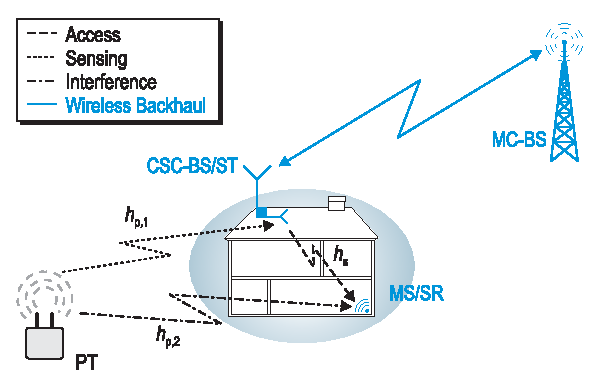
\includegraphics[width = 0.42 \paperwidth]{../figures/CR_Scenario_Interweave}
                }
        \end{center}
        \end{overlayarea}
        \only<1>{
                \fs{8}{8}
                Interweave System:
                \begin{itemize}
                        \item A spectrum sensing mechanism is employed at the ST.
                        \item To accomplish sensing $\Rightarrow$ Knowledge of the channel $\hpo$ is required. 
                        \item To characterize the throughput at SR $\Rightarrow$ Knowledge of the channels $\hpt, \hs$ is required. 
                \end{itemize}
                In a realistic scenario:
                \begin{itemize}
                \item \keyword{Issue:} Channel knowledge is not available at the ST. \keyword{Solution:} needs to be estimated.
                \item \keyword{Issue:} Conventional channel estimation techniques are incapable of sustaining requirements\footnote{Low-complexity and versatility towards unknown PU signals.} necessary for a hardware deployment of a CR system. \keyword{Solution:} Received power-based channel estimation is employed. 
                \end{itemize}
        }
        \only<2->{
                \fs{8}{8}
                Contributions:
                \begin{itemize}
                        \item Considering a deployment perspective, an analytical framework, proposed by Kaushik \textit{et al.}\footnote{Kaushik \textit{et al.}, ``Sensing-Throughput Tradeoff for Interweave Cognitive Radio System: A Deployment-Centric Viewpoint'', IEEE Transactions on Wireless Communications, Vol. 15, No. 5, May 2016, pp. 3690-3702.}, facilitating a successful incorporation of the estimation of the involved channels. 
                        \item We extend this analytical approach, where the interacting channels are subjected to Nakagami-$m$ fading.
			\item We depict an estimation-sensing-throughput tradeoff that allows us to optimize the performance of the interweave system.
                \end{itemize}
        }
\end{frame}


%%%%%%%%%%%%%%%%%%%%%%%%%%%%%%%%%%%%%%%%%%%%%%%%%%%% Frame %%%%%%%%%%%%%%%%%%%%%%%%%%%%%%%%%%%%%%%%%%%%%%%%%%%%%%       
\begin{frame}{System Model}
        \vspace{-0.8cm}
        \fs{8}{8}
        \begin{columns}[t]
                \begin{column}{0.51 \paperwidth}
                %\vspace{-0.4cm}
		\begin{center}
		\boxed{\mbox{ Signal Model}} 
		%\begin{theo}[Signal Model]
		\begin{itemize}
                     \item Received signal at the ST
                        \begin{equation*}
                        \yrcvd[n] = 
                                \begin{cases}
                                \hpo \cdot \xp[n] + w[n] & : \mathcal{H}_1 \\
                                w[n] & :\mathcal{H}_0
                                \end{cases}
                        \end{equation*}
                     \item Received signal at the SR
                        \begin{equation*}
                        \begin{cases}
                        \hs \cdot \xs[n] + \hpt \cdot \xp[n] + w[n] & : 1 - \pd \\
			\hs \cdot \xs[n] + w[n] & : 1 - \pfa
			\end{cases}
                        \end{equation*}
		  \end{itemize}
		%\end{theo}
                \end{center}
                \end{column}
                \begin{column}{0.49 \paperwidth}
                \begin{center}
		\boxed{\mbox{Interweave Scenario}} \\[0.3cm]
                        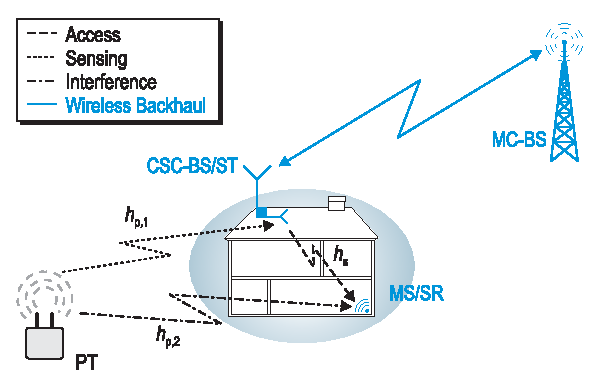
\includegraphics[width = 0.38 \paperwidth]{../figures/CR_Scenario_Interweave}
                \end{center}
                \end{column}
        \end{columns}
        \begin{columns}[t]
                \begin{column}{0.51 \paperwidth}
		\begin{center}
			\boxed{\mbox{(Symmetric) Channel fading}} \\[-0.4cm] 
			\begin{align*}
				\fphpo(x) = 1 - \Gamma\left(\mpo, \frac{\mpo x}{\bphpo}\right) \\  
				\fphpt(x) = 1 - \Gamma\left(\mpt, \frac{\mpt x}{\bphpt}\right) \\
				\fphs(x) = 1 - \Gamma\left(\ms , \frac{\ms x}{\bphs}\right) 
			\end{align*}
                \end{center}
                \end{column}
                \begin{column}{0.49 \paperwidth}
                \begin{center}
		\boxed{\mbox{Frame Structure}} \\[0.3cm]
                        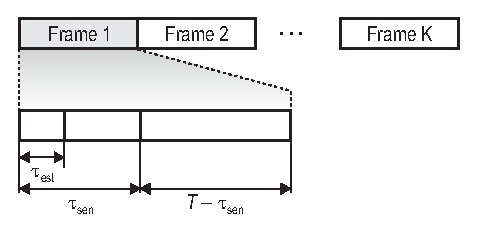
\includegraphics[width = 0.38 \paperwidth]{../figures/Frame_Structure_grau}
                \end{center}
                \end{column}
        \end{columns}
\end{frame}


%%%%%%%%%%%%%%%%%%%%%%%%%%%%%%%%%%%%%%%%%%%%%%%%%%%% Frame %%%%%%%%%%%%%%%%%%%%%%%%%%%%%%%%%%%%%%%%%%%%%%%%%%%%%%       
\begin{frame}{Perfect Channel Knowledge}
	\fs{8}{8}
                \begin{center}
		\begin{itemize}
                \item Performance parameters, including detection probability ($\pd$) and secondary throughput ($\rs$), observe variations due to channel fading. \\[0.1cm] 
                \end{itemize}
                \begin{mdframed}[style=MyFrame, frametitle=Ideal Model (IM)] \keyword{Problem 1}: Subject to an outage constraint on $\pd$, the sensing-throughput tradeoff that considers perfect channel estimation and random behaviour of the interacting channels, is given by
                \begin{align*}
               		\trsoc(\ttsenoc) &= \maxi_{\tsen} \e{\pd, \phs, \phpt}{\rs(\tsen)}, \\
			\text{s.t.} & \text{ }  \p( \pd \le \pdd) \le \mpd,  \\ 
			\text{s.t.} & \text{ }  0 < \tsen \le T, 
		\end{align*} \\[-0.6cm] 
		where\\[-0.7cm] 
		\begin{align*}
%\hspace{-8mm}
			\rs(\tsen) =& \frac{T - \tsen}{T} \mathbb{E}_{\phs \phpt} \bigg[ \phz (1 - \pfa) \smash[b]{\overbrace{\log_2 \bigg( 1 + \frac{\phs \ptranst}{\npo} \bigg)}^{\cz}} \\ &+ \pho (1 - \pd) \smash[b]{\overbrace{\log_2 \bigg( 1 + \frac{\phs \ptranst}{\phpt \ptranpt + \npo} \bigg)}^{\co}} \bigg]. 
			\end{align*}

		\end{mdframed}
                \end{center}
\end{frame}


%%%%%%%%%%%%%%%%%%%%%%%%%%%%%%%%%%%%%%%%%%%%%%%%%%%% Frame %%%%%%%%%%%%%%%%%%%%%%%%%%%%%%%%%%%%%%%%%%%%%%%%%%%%%%       
\begin{frame}{Perfect Channel Knowledge}
        \fs{8}{8}
                \begin{center}
                \begin{mdframed}[style=MyFrame, frametitle=Ideal Model (IM)] \keyword{Problem 1}: Subject to an outage constraint on $\pd$, the sensing-throughput tradeoff that considers perfect channel estimation and random behaviour of the interacting channels, is given by
                \begin{align*}
                        \trsoc(\ttsenoc) &= \maxi_{\tsen} \e{\pd, \phs, \phpt}{\rs(\tsen)}, \\
                        \text{s.t.} & \text{ }  \p( \pd \le \pdd) \le \mpd,  \\ 
                        \text{s.t.} & \text{ }  0 < \tsen \le T. 
                \end{align*} 
                \end{mdframed}
                \begin{itemize}
                \item \keyword{Issue:} Despite the knowledge of the fading model, the characterization of the secondary throughput and interference constraint assumes the perfect knowledge\footnote{This knowledge signifies the perfect knowledge of the different realizations of the corresponding channels.} of the power gains for the corresponding channels.
                \end{itemize}
                \end{center}
\end{frame}



%%%%%%%%%%%%%%%%%%%%%%%%%%%%%%%%%%%%%%%%%%%%%%%%%%%% Frame %%%%%%%%%%%%%%%%%%%%%%%%%%%%%%%%%%%%%%%%%%%%%%%%%%%%%%       
\begin{frame}{Imperfect Channel Knowledge}
	\fs{8}{8}
                \begin{center}
		\begin{itemize}
                \item Performance parameters observe variations due to channel estimation and channel fading. 
                \item The variations due to channel estimation in the performance parameters ($\epd$ and ($\eco, \ecz$)) have been characterized in Kaushik \textit{et al.}. 
		\item Interference constraint to encounter uncertain interference: 
                \end{itemize}
		\begin{align*}
			\smash[b]{\underbrace{\mathbb{E}_{\phpo}{\smash[b]{\overbrace{[\p( \epd \le \pdd)]}^{\text{Channel Estimation}}}}}_{\text{Channel fading}}} &\le \mpd \\[0.2cm] 
\end{align*}

		\begin{mdframed}[style=MyFrame, frametitle=Estimation Model (EM)] \keyword{Problem 2}: Subject to an outage constraint on $\pd$, the sensing-throughput tradeoff that considers imperfect channel estimation and random behaviour of the interacting channels, is given by
                \begin{align*}
			\trsoc(\ttest, \ttsen) &= \maxi_{\test, \tsen} \e{\epd, \ecz, \eco, \phpo, \phs, \phpt}{\rs(\test, \tsen)}, \nonumber \\ 
			\text{s.t.} & \text{ }  \mathbb{E}_{\phpo}\p( \epd \le \pdd)  \le \mpd, \\
			\text{s.t.} & \text{ }  0 < \test \le \tsen \le T.
		\end{align*}
		\end{mdframed}
                \end{center}
\end{frame}


%%%%%%%%%%%%%%%%%%%%%%%%%%%%%%%%%%%%%%%%%%%%%%%%%%%%% Frame %%%%%%%%%%%%%%%%%%%%%%%%%%%%%%%%%%%%%%%%%%%%%%%%%%%%%%
\begin{frame}{Numerical Analysis}
\vspace{-0.2cm}
\fs{8}{8}
\begin{center}
\renewcommand{\arraystretch}{1.35}
\begin{tabular}{c||c|c}
\bfseries Parameter & \bfseries Definition & \bfseries Value \\
\hline\hline
$\fsam$ & Sampling Frequency & $\SI{1}{MHz}$ \\ \hline
$T$ & Frame duration & $\SI{100}{ms}$ \\ \hline
$\bphpo$ & Sensing channel gain & $\SI{-100}{dB}$ \\ \hline
$\bphpt$ & Interference channel gain & $\SI{-100}{dB}$ \\ \hline
$\bphs$ & Access channel gain & $\SI{-80}{dB}$ \\ \hline 
$\pdd$ & Target detection probability & 0.9 \\ \hline 
$\mpd$ & Outage constraint & 0.05  \\ \hline 
$\npo$ & Noise power & $\SI{-100}{dBm}$ \\ \hline
$\snrrcvd$ & Signal to noise ratio at ST over $\hpo$ & $\SI{-10}{dB}$ \\ \hline
$\snrpt$ & Signal to noise ratio at PT over $\hpt$ & $\SI{-10}{dB}$ \\ \hline
$\snrso$ & Signal to noise ratio at SR over $\hs$ & $\SI{10}{dB}$ \\ \hline
$\spo = \ptranpt$ & Transmit power at PT &$-\SI{10}{dBm}$ \\ \hline
$\ptranst$ &Transmit power at ST & $-\SI{10}{dBm}$ \\ \hline
$\pho$ &  Occurrence probability of hypothesis $\mathcal H_1$ & 0.2 \\ \hline
$\test$ & Estimation time & $\SI{1}{ms}$ \\ \hline
$\Ks$ & Number of pilot symbols &10 \\ \hline 
$m$& Nakagami-$m$ parameter & $\{1, 1.5\}$  
\end{tabular}
\end{center}
\end{frame}

%%%%%%%%%%%%%%%%%%%%%%%%%%%%%%%%%%%%%%%%%%%%%%%%%%%%% Frame %%%%%%%%%%%%%%%%%%%%%%%%%%%%%%%%%%%%%%%%%%%%%%%%%%%%%%
\begin{frame}[t]{Numerical Analysis}
        \begin{overlayarea}{\textwidth}{6.0cm}
        \begin{center}
                \fs{8}{8}
                \boxed{\mbox{Sensing-throughput tradeoff}} \\
		\resizebox{0.55\textwidth}{!}{%
		% This file is generated by the MATLAB m-file laprint.m. It can be included
% into LaTeX documents using the packages graphicx, color and psfrag.
% It is accompanied by a postscript file. A sample LaTeX file is:
%    \documentclass{article}\usepackage{graphicx,color,psfrag}
%    \begin{document}% This file is generated by the MATLAB m-file laprint.m. It can be included
% into LaTeX documents using the packages graphicx, color and psfrag.
% It is accompanied by a postscript file. A sample LaTeX file is:
%    \documentclass{article}\usepackage{graphicx,color,psfrag}
%    \begin{document}% This file is generated by the MATLAB m-file laprint.m. It can be included
% into LaTeX documents using the packages graphicx, color and psfrag.
% It is accompanied by a postscript file. A sample LaTeX file is:
%    \documentclass{article}\usepackage{graphicx,color,psfrag}
%    \begin{document}\input{fig_thr_sen_time_tradeoff_fading}\end{document}
% See http://www.mathworks.de/matlabcentral/fileexchange/loadFile.do?objectId=4638
% for recent versions of laprint.m.
%
% created by:           LaPrint version 3.16 (13.9.2004)
% created on:           12-Jul-2016 15:14:00
% eps bounding box:     16 cm x 12 cm
% comment:              
%
%\begin{psfrags}%
%\psfragscanon%
%
% text strings:
\psfrag{s05}[b][b]{\fontsize{8}{12}\fontseries{m}\mathversion{normal}\fontshape{n}\selectfont \color[rgb]{0,0,0}\setlength{\tabcolsep}{0pt}\begin{tabular}{c}$\rs(\test = \SI{1}{ms}, \tsen)$ [bits/sec/Hz]\end{tabular}}%
\psfrag{s06}[t][t]{\fontsize{8}{12}\fontseries{m}\mathversion{normal}\fontshape{n}\selectfont \color[rgb]{0,0,0}\setlength{\tabcolsep}{0pt}\begin{tabular}{c}$\tsen$ [ms]\end{tabular}}%
\psfrag{s10}[][]{\fontsize{10}{15}\fontseries{m}\mathversion{normal}\fontshape{n}\selectfont \color[rgb]{0,0,0}\setlength{\tabcolsep}{0pt}\begin{tabular}{c} \end{tabular}}%
\psfrag{s11}[][]{\fontsize{10}{15}\fontseries{m}\mathversion{normal}\fontshape{n}\selectfont \color[rgb]{0,0,0}\setlength{\tabcolsep}{0pt}\begin{tabular}{c} \end{tabular}}%
\psfrag{s12}[l][l]{\fontsize{8}{12}\fontseries{m}\mathversion{normal}\fontshape{n}\selectfont \color[rgb]{0,0,0}Simulated}%
\psfrag{s13}[l][l]{\fontsize{8}{12}\fontseries{m}\mathversion{normal}\fontshape{n}\selectfont \color[rgb]{0,0,0}IM, Problem 1}%
\psfrag{s14}[l][l]{\fontsize{8}{12}\fontseries{m}\mathversion{normal}\fontshape{n}\selectfont \color[rgb]{0,0,0}EM, Problem 2}%
\psfrag{s15}[l][l]{\fontsize{8}{12}\fontseries{m}\mathversion{normal}\fontshape{n}\selectfont \color[rgb]{0,0,0}$\trs(\test,\ttsen)$}%
\psfrag{s16}[l][l]{\fontsize{8}{12}\fontseries{m}\mathversion{normal}\fontshape{n}\selectfont \color[rgb]{0,0,0}Simulated}%
%
% axes font properties:
\fontsize{8}{12}\fontseries{m}\mathversion{normal}%
\fontshape{n}\selectfont%
%
% xticklabels:
\psfrag{x01}[t][t]{0}%
\psfrag{x02}[t][t]{5}%
\psfrag{x03}[t][t]{10}%
\psfrag{x04}[t][t]{15}%
%
% yticklabels:
\psfrag{v01}[r][r]{0}%
\psfrag{v02}[r][r]{0.5}%
\psfrag{v03}[r][r]{1}%
\psfrag{v04}[r][r]{1.5}%
\psfrag{v05}[r][r]{2}%
%
% Figure:
%\resizebox{8cm}{!}{\includegraphics{fig_thr_sen_time_tradeoff_fading.eps}}%
%\end{psfrags}%
%
% End fig_thr_sen_time_tradeoff_fading.tex
\end{document}
% See http://www.mathworks.de/matlabcentral/fileexchange/loadFile.do?objectId=4638
% for recent versions of laprint.m.
%
% created by:           LaPrint version 3.16 (13.9.2004)
% created on:           12-Jul-2016 15:14:00
% eps bounding box:     16 cm x 12 cm
% comment:              
%
%\begin{psfrags}%
%\psfragscanon%
%
% text strings:
\psfrag{s05}[b][b]{\fontsize{8}{12}\fontseries{m}\mathversion{normal}\fontshape{n}\selectfont \color[rgb]{0,0,0}\setlength{\tabcolsep}{0pt}\begin{tabular}{c}$\rs(\test = \SI{1}{ms}, \tsen)$ [bits/sec/Hz]\end{tabular}}%
\psfrag{s06}[t][t]{\fontsize{8}{12}\fontseries{m}\mathversion{normal}\fontshape{n}\selectfont \color[rgb]{0,0,0}\setlength{\tabcolsep}{0pt}\begin{tabular}{c}$\tsen$ [ms]\end{tabular}}%
\psfrag{s10}[][]{\fontsize{10}{15}\fontseries{m}\mathversion{normal}\fontshape{n}\selectfont \color[rgb]{0,0,0}\setlength{\tabcolsep}{0pt}\begin{tabular}{c} \end{tabular}}%
\psfrag{s11}[][]{\fontsize{10}{15}\fontseries{m}\mathversion{normal}\fontshape{n}\selectfont \color[rgb]{0,0,0}\setlength{\tabcolsep}{0pt}\begin{tabular}{c} \end{tabular}}%
\psfrag{s12}[l][l]{\fontsize{8}{12}\fontseries{m}\mathversion{normal}\fontshape{n}\selectfont \color[rgb]{0,0,0}Simulated}%
\psfrag{s13}[l][l]{\fontsize{8}{12}\fontseries{m}\mathversion{normal}\fontshape{n}\selectfont \color[rgb]{0,0,0}IM, Problem 1}%
\psfrag{s14}[l][l]{\fontsize{8}{12}\fontseries{m}\mathversion{normal}\fontshape{n}\selectfont \color[rgb]{0,0,0}EM, Problem 2}%
\psfrag{s15}[l][l]{\fontsize{8}{12}\fontseries{m}\mathversion{normal}\fontshape{n}\selectfont \color[rgb]{0,0,0}$\trs(\test,\ttsen)$}%
\psfrag{s16}[l][l]{\fontsize{8}{12}\fontseries{m}\mathversion{normal}\fontshape{n}\selectfont \color[rgb]{0,0,0}Simulated}%
%
% axes font properties:
\fontsize{8}{12}\fontseries{m}\mathversion{normal}%
\fontshape{n}\selectfont%
%
% xticklabels:
\psfrag{x01}[t][t]{0}%
\psfrag{x02}[t][t]{5}%
\psfrag{x03}[t][t]{10}%
\psfrag{x04}[t][t]{15}%
%
% yticklabels:
\psfrag{v01}[r][r]{0}%
\psfrag{v02}[r][r]{0.5}%
\psfrag{v03}[r][r]{1}%
\psfrag{v04}[r][r]{1.5}%
\psfrag{v05}[r][r]{2}%
%
% Figure:
%\resizebox{8cm}{!}{\includegraphics{fig_thr_sen_time_tradeoff_fading.eps}}%
%\end{psfrags}%
%
% End fig_thr_sen_time_tradeoff_fading.tex
\end{document}
% See http://www.mathworks.de/matlabcentral/fileexchange/loadFile.do?objectId=4638
% for recent versions of laprint.m.
%
% created by:           LaPrint version 3.16 (13.9.2004)
% created on:           12-Jul-2016 15:14:00
% eps bounding box:     16 cm x 12 cm
% comment:              
%
%\begin{psfrags}%
%\psfragscanon%
%
% text strings:
\psfrag{s05}[b][b]{\fontsize{8}{12}\fontseries{m}\mathversion{normal}\fontshape{n}\selectfont \color[rgb]{0,0,0}\setlength{\tabcolsep}{0pt}\begin{tabular}{c}$\rs(\test = \SI{1}{ms}, \tsen)$ [bits/sec/Hz]\end{tabular}}%
\psfrag{s06}[t][t]{\fontsize{8}{12}\fontseries{m}\mathversion{normal}\fontshape{n}\selectfont \color[rgb]{0,0,0}\setlength{\tabcolsep}{0pt}\begin{tabular}{c}$\tsen$ [ms]\end{tabular}}%
\psfrag{s10}[][]{\fontsize{10}{15}\fontseries{m}\mathversion{normal}\fontshape{n}\selectfont \color[rgb]{0,0,0}\setlength{\tabcolsep}{0pt}\begin{tabular}{c} \end{tabular}}%
\psfrag{s11}[][]{\fontsize{10}{15}\fontseries{m}\mathversion{normal}\fontshape{n}\selectfont \color[rgb]{0,0,0}\setlength{\tabcolsep}{0pt}\begin{tabular}{c} \end{tabular}}%
\psfrag{s12}[l][l]{\fontsize{8}{12}\fontseries{m}\mathversion{normal}\fontshape{n}\selectfont \color[rgb]{0,0,0}Simulated}%
\psfrag{s13}[l][l]{\fontsize{8}{12}\fontseries{m}\mathversion{normal}\fontshape{n}\selectfont \color[rgb]{0,0,0}IM, Problem 1}%
\psfrag{s14}[l][l]{\fontsize{8}{12}\fontseries{m}\mathversion{normal}\fontshape{n}\selectfont \color[rgb]{0,0,0}EM, Problem 2}%
\psfrag{s15}[l][l]{\fontsize{8}{12}\fontseries{m}\mathversion{normal}\fontshape{n}\selectfont \color[rgb]{0,0,0}$\trs(\test,\ttsen)$}%
\psfrag{s16}[l][l]{\fontsize{8}{12}\fontseries{m}\mathversion{normal}\fontshape{n}\selectfont \color[rgb]{0,0,0}Simulated}%
%
% axes font properties:
\fontsize{8}{12}\fontseries{m}\mathversion{normal}%
\fontshape{n}\selectfont%
%
% xticklabels:
\psfrag{x01}[t][t]{0}%
\psfrag{x02}[t][t]{5}%
\psfrag{x03}[t][t]{10}%
\psfrag{x04}[t][t]{15}%
%
% yticklabels:
\psfrag{v01}[r][r]{0}%
\psfrag{v02}[r][r]{0.5}%
\psfrag{v03}[r][r]{1}%
\psfrag{v04}[r][r]{1.5}%
\psfrag{v05}[r][r]{2}%
%
% Figure:
%\resizebox{8cm}{!}{\includegraphics{fig_thr_sen_time_tradeoff_fading.eps}}%
%\end{psfrags}%
%
% End fig_thr_sen_time_tradeoff_fading.tex

		\begin{tikzpicture}[scale=1]
		\node[anchor=south west,inner sep=0] (image) at (0,0)
		{
  			\includegraphics[width= \figscale]{../figures/fig_thr_sen_time_tradeoff_fading}
		};
		\begin{scope}[x={(image.south east)},y={(image.north west)}]

		%\node[draw,fill=gray!10,font=\small] (senid) at (0.232,0.83) {$\trs$};
		%\draw[black, ->] (senid.north) -- (0.232,0.93);
		%\node[draw,fill=gray!10,font=\small] (senac) at (0.378,0.882) {$\trsac$};
		%\draw[black, ->] (senac.east) -- (0.478,0.882);
		%\node[draw,fill=gray!10,font=\small] (senoc) at (0.614,0.733) {$\trsoc$};
		%\draw[black, ->] (senoc.north) -- (0.614,0.833);

		\draw[black,thick,<->] (0.082,0.12) --  node[above, font=\scriptsize] {$\test$} (0.14,0.12);
		\draw (0.82,0.8) arc(-160:160:0.007 and 0.021);
		\node[draw, fill=gray!10, font=\scriptsize] (text4) at (0.72,0.74) {$m = 1$};
		\draw[black, ->] (text4.east) -- (0.82,0.795);

		\draw (0.38,0.907) arc(-160:160:0.007 and 0.021);
		\node[draw, fill=gray!10, font=\scriptsize] (text5) at (0.27,0.847) {$m = 1.5$};
		\draw[black, ->] (text5.east) -- (0.38,0.902);

		%\draw[help lines,xstep=.1,ystep=.1] (0,0) grid (1,1);
		%\foreach \x in {0,1,...,9} { \node [anchor=north] at (\x/10,0) {0.\x}; }
		%\foreach \y in {0,1,...,9} { \node [anchor=east] at (0,\y/10) {0.\y}; }
		\end{scope}
		\end{tikzpicture}
		}
        \end{center}
        \end{overlayarea}
        \fs{8}{8}
        \begin{itemize}
                \item EM procures no secondary throughput for the estimation time. 
                \item Suitable sensing time increases with severity in fading. 
        \end{itemize}
\end{frame}


%%%%%%%%%%%%%%%%%%%%%%%%%%%%%%%%%%%%%%%%%%%%%%%%%%%%% Frame %%%%%%%%%%%%%%%%%%%%%%%%%%%%%%%%%%%%%%%%%%%%%%%%%%%%%%
\begin{frame}[t]{Numerical Analysis}
        \begin{overlayarea}{\textwidth}{6.0cm}
        \begin{center}
                \fs{8}{8}
                \boxed{\mbox{Estimation-sensing-throughput tradeoff}} \\
		\resizebox{0.55\textwidth}{!}{%
		% This file is generated by the MATLAB m-file laprint.m. It can be included
% into LaTeX documents using the packages graphicx, color and psfrag.
% It is accompanied by a postscript file. A sample LaTeX file is:
%    \documentclass{article}\usepackage{graphicx,color,psfrag}
%    \begin{document}% This file is generated by the MATLAB m-file laprint.m. It can be included
% into LaTeX documents using the packages graphicx, color and psfrag.
% It is accompanied by a postscript file. A sample LaTeX file is:
%    \documentclass{article}\usepackage{graphicx,color,psfrag}
%    \begin{document}% This file is generated by the MATLAB m-file laprint.m. It can be included
% into LaTeX documents using the packages graphicx, color and psfrag.
% It is accompanied by a postscript file. A sample LaTeX file is:
%    \documentclass{article}\usepackage{graphicx,color,psfrag}
%    \begin{document}\input{fig_opt_thr_vs_est_time_fading}\end{document}
% See http://www.mathworks.de/matlabcentral/fileexchange/loadFile.do?objectId=4638
% for recent versions of laprint.m.
%
% created by:           LaPrint version 3.16 (13.9.2004)
% created on:           12-Jul-2016 15:25:44
% eps bounding box:     16 cm x 12 cm
% comment:              
%
%\begin{psfrags}%
%\psfragscanon%
%
% text strings:
\psfrag{s05}[b][b]{\fontsize{8}{12}\fontseries{m}\mathversion{normal}\fontshape{n}\selectfont \color[rgb]{0,0,0}\setlength{\tabcolsep}{0pt}\begin{tabular}{c}$\rs(\test,\ttsen)$\end{tabular}}%
\psfrag{s06}[t][t]{\fontsize{8}{12}\fontseries{m}\mathversion{normal}\fontshape{n}\selectfont \color[rgb]{0,0,0}\setlength{\tabcolsep}{0pt}\begin{tabular}{c}$\test$ [ms]\end{tabular}}%
\psfrag{s10}[][]{\fontsize{10}{15}\fontseries{m}\mathversion{normal}\fontshape{n}\selectfont \color[rgb]{0,0,0}\setlength{\tabcolsep}{0pt}\begin{tabular}{c} \end{tabular}}%
\psfrag{s11}[][]{\fontsize{10}{15}\fontseries{m}\mathversion{normal}\fontshape{n}\selectfont \color[rgb]{0,0,0}\setlength{\tabcolsep}{0pt}\begin{tabular}{c} \end{tabular}}%
\psfrag{s12}[l][l]{\fontsize{8}{12}\fontseries{m}\mathversion{normal}\fontshape{n}\selectfont \color[rgb]{0,0,0}$\trs(\ttest,\ttsen)$}%
\psfrag{s13}[l][l]{\fontsize{8}{12}\fontseries{m}\mathversion{normal}\fontshape{n}\selectfont \color[rgb]{0,0,0}IM, Problem 1}%
\psfrag{s14}[l][l]{\fontsize{8}{12}\fontseries{m}\mathversion{normal}\fontshape{n}\selectfont \color[rgb]{0,0,0}EM, Problem 2}%
\psfrag{s15}[l][l]{\fontsize{8}{12}\fontseries{m}\mathversion{normal}\fontshape{n}\selectfont \color[rgb]{0,0,0}$\trs(\ttest,\ttsen)$}%
%
% axes font properties:
\fontsize{8}{12}\fontseries{m}\mathversion{normal}%
\fontshape{n}\selectfont%
%
% xticklabels:
\psfrag{x01}[t][t]{1}%
\psfrag{x02}[t][t]{2}%
\psfrag{x03}[t][t]{3}%
\psfrag{x04}[t][t]{4}%
\psfrag{x05}[t][t]{5}%
\psfrag{x06}[t][t]{6}%
\psfrag{x07}[t][t]{7}%
\psfrag{x08}[t][t]{8}%
\psfrag{x09}[t][t]{9}%
\psfrag{x10}[t][t]{10}%
\psfrag{x11}[t][t]{11}%
\psfrag{x12}[t][t]{12}%
%
% yticklabels:
\psfrag{v01}[r][r]{1}%
\psfrag{v02}[r][r]{1.2}%
\psfrag{v03}[r][r]{1.4}%
\psfrag{v04}[r][r]{1.6}%
\psfrag{v05}[r][r]{1.8}%
\psfrag{v06}[r][r]{2}%
\psfrag{v07}[r][r]{2.2}%
\psfrag{v08}[r][r]{2.4}%
%
% Figure:
%\resizebox{8cm}{!}{\includegraphics{fig_opt_thr_vs_est_time_fading.eps}}%
%\end{psfrags}%
%
% End fig_opt_thr_vs_est_time_fading.tex
\end{document}
% See http://www.mathworks.de/matlabcentral/fileexchange/loadFile.do?objectId=4638
% for recent versions of laprint.m.
%
% created by:           LaPrint version 3.16 (13.9.2004)
% created on:           12-Jul-2016 15:25:44
% eps bounding box:     16 cm x 12 cm
% comment:              
%
%\begin{psfrags}%
%\psfragscanon%
%
% text strings:
\psfrag{s05}[b][b]{\fontsize{8}{12}\fontseries{m}\mathversion{normal}\fontshape{n}\selectfont \color[rgb]{0,0,0}\setlength{\tabcolsep}{0pt}\begin{tabular}{c}$\rs(\test,\ttsen)$\end{tabular}}%
\psfrag{s06}[t][t]{\fontsize{8}{12}\fontseries{m}\mathversion{normal}\fontshape{n}\selectfont \color[rgb]{0,0,0}\setlength{\tabcolsep}{0pt}\begin{tabular}{c}$\test$ [ms]\end{tabular}}%
\psfrag{s10}[][]{\fontsize{10}{15}\fontseries{m}\mathversion{normal}\fontshape{n}\selectfont \color[rgb]{0,0,0}\setlength{\tabcolsep}{0pt}\begin{tabular}{c} \end{tabular}}%
\psfrag{s11}[][]{\fontsize{10}{15}\fontseries{m}\mathversion{normal}\fontshape{n}\selectfont \color[rgb]{0,0,0}\setlength{\tabcolsep}{0pt}\begin{tabular}{c} \end{tabular}}%
\psfrag{s12}[l][l]{\fontsize{8}{12}\fontseries{m}\mathversion{normal}\fontshape{n}\selectfont \color[rgb]{0,0,0}$\trs(\ttest,\ttsen)$}%
\psfrag{s13}[l][l]{\fontsize{8}{12}\fontseries{m}\mathversion{normal}\fontshape{n}\selectfont \color[rgb]{0,0,0}IM, Problem 1}%
\psfrag{s14}[l][l]{\fontsize{8}{12}\fontseries{m}\mathversion{normal}\fontshape{n}\selectfont \color[rgb]{0,0,0}EM, Problem 2}%
\psfrag{s15}[l][l]{\fontsize{8}{12}\fontseries{m}\mathversion{normal}\fontshape{n}\selectfont \color[rgb]{0,0,0}$\trs(\ttest,\ttsen)$}%
%
% axes font properties:
\fontsize{8}{12}\fontseries{m}\mathversion{normal}%
\fontshape{n}\selectfont%
%
% xticklabels:
\psfrag{x01}[t][t]{1}%
\psfrag{x02}[t][t]{2}%
\psfrag{x03}[t][t]{3}%
\psfrag{x04}[t][t]{4}%
\psfrag{x05}[t][t]{5}%
\psfrag{x06}[t][t]{6}%
\psfrag{x07}[t][t]{7}%
\psfrag{x08}[t][t]{8}%
\psfrag{x09}[t][t]{9}%
\psfrag{x10}[t][t]{10}%
\psfrag{x11}[t][t]{11}%
\psfrag{x12}[t][t]{12}%
%
% yticklabels:
\psfrag{v01}[r][r]{1}%
\psfrag{v02}[r][r]{1.2}%
\psfrag{v03}[r][r]{1.4}%
\psfrag{v04}[r][r]{1.6}%
\psfrag{v05}[r][r]{1.8}%
\psfrag{v06}[r][r]{2}%
\psfrag{v07}[r][r]{2.2}%
\psfrag{v08}[r][r]{2.4}%
%
% Figure:
%\resizebox{8cm}{!}{\includegraphics{fig_opt_thr_vs_est_time_fading.eps}}%
%\end{psfrags}%
%
% End fig_opt_thr_vs_est_time_fading.tex
\end{document}
% See http://www.mathworks.de/matlabcentral/fileexchange/loadFile.do?objectId=4638
% for recent versions of laprint.m.
%
% created by:           LaPrint version 3.16 (13.9.2004)
% created on:           12-Jul-2016 15:25:44
% eps bounding box:     16 cm x 12 cm
% comment:              
%
%\begin{psfrags}%
%\psfragscanon%
%
% text strings:
\psfrag{s05}[b][b]{\fontsize{8}{12}\fontseries{m}\mathversion{normal}\fontshape{n}\selectfont \color[rgb]{0,0,0}\setlength{\tabcolsep}{0pt}\begin{tabular}{c}$\rs(\test,\ttsen)$\end{tabular}}%
\psfrag{s06}[t][t]{\fontsize{8}{12}\fontseries{m}\mathversion{normal}\fontshape{n}\selectfont \color[rgb]{0,0,0}\setlength{\tabcolsep}{0pt}\begin{tabular}{c}$\test$ [ms]\end{tabular}}%
\psfrag{s10}[][]{\fontsize{10}{15}\fontseries{m}\mathversion{normal}\fontshape{n}\selectfont \color[rgb]{0,0,0}\setlength{\tabcolsep}{0pt}\begin{tabular}{c} \end{tabular}}%
\psfrag{s11}[][]{\fontsize{10}{15}\fontseries{m}\mathversion{normal}\fontshape{n}\selectfont \color[rgb]{0,0,0}\setlength{\tabcolsep}{0pt}\begin{tabular}{c} \end{tabular}}%
\psfrag{s12}[l][l]{\fontsize{8}{12}\fontseries{m}\mathversion{normal}\fontshape{n}\selectfont \color[rgb]{0,0,0}$\trs(\ttest,\ttsen)$}%
\psfrag{s13}[l][l]{\fontsize{8}{12}\fontseries{m}\mathversion{normal}\fontshape{n}\selectfont \color[rgb]{0,0,0}IM, Problem 1}%
\psfrag{s14}[l][l]{\fontsize{8}{12}\fontseries{m}\mathversion{normal}\fontshape{n}\selectfont \color[rgb]{0,0,0}EM, Problem 2}%
\psfrag{s15}[l][l]{\fontsize{8}{12}\fontseries{m}\mathversion{normal}\fontshape{n}\selectfont \color[rgb]{0,0,0}$\trs(\ttest,\ttsen)$}%
%
% axes font properties:
\fontsize{8}{12}\fontseries{m}\mathversion{normal}%
\fontshape{n}\selectfont%
%
% xticklabels:
\psfrag{x01}[t][t]{1}%
\psfrag{x02}[t][t]{2}%
\psfrag{x03}[t][t]{3}%
\psfrag{x04}[t][t]{4}%
\psfrag{x05}[t][t]{5}%
\psfrag{x06}[t][t]{6}%
\psfrag{x07}[t][t]{7}%
\psfrag{x08}[t][t]{8}%
\psfrag{x09}[t][t]{9}%
\psfrag{x10}[t][t]{10}%
\psfrag{x11}[t][t]{11}%
\psfrag{x12}[t][t]{12}%
%
% yticklabels:
\psfrag{v01}[r][r]{1}%
\psfrag{v02}[r][r]{1.2}%
\psfrag{v03}[r][r]{1.4}%
\psfrag{v04}[r][r]{1.6}%
\psfrag{v05}[r][r]{1.8}%
\psfrag{v06}[r][r]{2}%
\psfrag{v07}[r][r]{2.2}%
\psfrag{v08}[r][r]{2.4}%
%
% Figure:
%\resizebox{8cm}{!}{\includegraphics{fig_opt_thr_vs_est_time_fading.eps}}%
%\end{psfrags}%
%
% End fig_opt_thr_vs_est_time_fading.tex

		\centering
		\begin{tikzpicture}[scale=1]
			\node[anchor=south west,inner sep=0] (image) at (0,0)
			{
				\includegraphics[width= \figscale]{../figures/fig_opt_thr_vs_est_time_fading.eps}
			};
			\begin{scope}[x={(image.south east)},y={(image.north west)}]


			\draw (0.54,0.74) arc(-160:160:0.007 and 0.021);
			\node[draw, fill=gray!10, font=\scriptsize] (text4) at (0.44,0.68) {$m = 1$};
			\draw[black, ->] (text4.east) -- (0.54,0.735);

			\draw (0.3,0.92) arc(-160:160:0.009 and 0.027);
			\node[draw, fill=gray!10, font=\scriptsize] (text5) at (0.19,0.86) {$m = 1.5$};
			\draw[black, ->] (text5.east) -- (0.302,0.913);


			%%\draw[help lines,xstep=.1,ystep=.1] (0,0) grid (1,1);
			%%\foreach \x in {0,1,...,9} { \node [anchor=north] at (\x/10,0) {0.\x}; }
			%%\foreach \y in {0,1,...,9} { \node [anchor=east] at (0,\y/10) {0.\y}; }
			\end{scope}
		\end{tikzpicture}
	}
        \end{center}
        \end{overlayarea}
        \fs{8}{8}
        \begin{itemize}
                \item $\rs(\test, \ttsen)$ increases for low values of $\test$ and then decreases beyond $\ttest$.
                \item While comparing IM and EM, it is obseved that the mild fading scenarios (e.g. $m = 1.5$) are more sensitive to the performance degradation. 
        \end{itemize}
\end{frame}


%%%%%%%%%%%%%%%%%%%%%%%%%%%%%%%%%%%%%%%%%%%%%%%%%%%%% Frame %%%%%%%%%%%%%%%%%%%%%%%%%%%%%%%%%%%%%%%%%%%%%%%%%%%%%%
\begin{frame}[t]{Numerical Analysis}
        \begin{overlayarea}{\textwidth}{6.0cm}
        \begin{center}
                \fs{8}{8}
                \boxed{\mbox{Expected detection probability vs estimation time}} \\
		\resizebox{0.55\textwidth}{!}{%
			% This file is generated by the MATLAB m-file laprint.m. It can be included
% into LaTeX documents using the packages graphicx, color and psfrag.
% It is accompanied by a postscript file. A sample LaTeX file is:
%    \documentclass{article}\usepackage{graphicx,color,psfrag}
%    \begin{document}% This file is generated by the MATLAB m-file laprint.m. It can be included
% into LaTeX documents using the packages graphicx, color and psfrag.
% It is accompanied by a postscript file. A sample LaTeX file is:
%    \documentclass{article}\usepackage{graphicx,color,psfrag}
%    \begin{document}% This file is generated by the MATLAB m-file laprint.m. It can be included
% into LaTeX documents using the packages graphicx, color and psfrag.
% It is accompanied by a postscript file. A sample LaTeX file is:
%    \documentclass{article}\usepackage{graphicx,color,psfrag}
%    \begin{document}\input{fig_P_d_vs_est_time_fading}\end{document}
% See http://www.mathworks.de/matlabcentral/fileexchange/loadFile.do?objectId=4638
% for recent versions of laprint.m.
%
% created by:           LaPrint version 3.16 (13.9.2004)
% created on:           12-Jul-2016 15:25:47
% eps bounding box:     16 cm x 12 cm
% comment:              
%
%\begin{psfrags}%
%\psfragscanon%
%
% text strings:
\psfrag{s05}[b][b]{\fontsize{8}{12}\fontseries{m}\mathversion{normal}\fontshape{n}\selectfont \color[rgb]{0,0,0}\setlength{\tabcolsep}{0pt}\begin{tabular}{c}$\e{\epd, \phpo}{\epd}$\end{tabular}}%
\psfrag{s06}[t][t]{\fontsize{8}{12}\fontseries{m}\mathversion{normal}\fontshape{n}\selectfont \color[rgb]{0,0,0}\setlength{\tabcolsep}{0pt}\begin{tabular}{c}$\test$ [ms]\end{tabular}}%
\psfrag{s10}[][]{\fontsize{10}{15}\fontseries{m}\mathversion{normal}\fontshape{n}\selectfont \color[rgb]{0,0,0}\setlength{\tabcolsep}{0pt}\begin{tabular}{c} \end{tabular}}%
\psfrag{s11}[][]{\fontsize{10}{15}\fontseries{m}\mathversion{normal}\fontshape{n}\selectfont \color[rgb]{0,0,0}\setlength{\tabcolsep}{0pt}\begin{tabular}{c} \end{tabular}}%
\psfrag{s12}[l][l]{\fontsize{8}{12}\fontseries{m}\mathversion{normal}\fontshape{n}\selectfont \color[rgb]{0,0,0}EM, Problem 2}%
\psfrag{s13}[l][l]{\fontsize{8}{12}\fontseries{m}\mathversion{normal}\fontshape{n}\selectfont \color[rgb]{0,0,0}IM, Problem 1}%
\psfrag{s14}[l][l]{\fontsize{8}{12}\fontseries{m}\mathversion{normal}\fontshape{n}\selectfont \color[rgb]{0,0,0}EM, Problem 2}%
%
% axes font properties:
\fontsize{8}{12}\fontseries{m}\mathversion{normal}%
\fontshape{n}\selectfont%
%
% xticklabels:
\psfrag{x01}[t][t]{1}%
\psfrag{x02}[t][t]{2}%
\psfrag{x03}[t][t]{3}%
\psfrag{x04}[t][t]{4}%
\psfrag{x05}[t][t]{5}%
\psfrag{x06}[t][t]{6}%
\psfrag{x07}[t][t]{7}%
\psfrag{x08}[t][t]{8}%
\psfrag{x09}[t][t]{9}%
\psfrag{x10}[t][t]{10}%
\psfrag{x11}[t][t]{11}%
\psfrag{x12}[t][t]{12}%
%
% yticklabels:
\psfrag{v01}[r][r]{0.95}%
\psfrag{v02}[r][r]{0.96}%
\psfrag{v03}[r][r]{0.97}%
\psfrag{v04}[r][r]{0.98}%
%
% Figure:
%\resizebox{8cm}{!}{\includegraphics{fig_P_d_vs_est_time_fading.eps}}%
%\end{psfrags}%
%
% End fig_P_d_vs_est_time_fading.tex
\end{document}
% See http://www.mathworks.de/matlabcentral/fileexchange/loadFile.do?objectId=4638
% for recent versions of laprint.m.
%
% created by:           LaPrint version 3.16 (13.9.2004)
% created on:           12-Jul-2016 15:25:47
% eps bounding box:     16 cm x 12 cm
% comment:              
%
%\begin{psfrags}%
%\psfragscanon%
%
% text strings:
\psfrag{s05}[b][b]{\fontsize{8}{12}\fontseries{m}\mathversion{normal}\fontshape{n}\selectfont \color[rgb]{0,0,0}\setlength{\tabcolsep}{0pt}\begin{tabular}{c}$\e{\epd, \phpo}{\epd}$\end{tabular}}%
\psfrag{s06}[t][t]{\fontsize{8}{12}\fontseries{m}\mathversion{normal}\fontshape{n}\selectfont \color[rgb]{0,0,0}\setlength{\tabcolsep}{0pt}\begin{tabular}{c}$\test$ [ms]\end{tabular}}%
\psfrag{s10}[][]{\fontsize{10}{15}\fontseries{m}\mathversion{normal}\fontshape{n}\selectfont \color[rgb]{0,0,0}\setlength{\tabcolsep}{0pt}\begin{tabular}{c} \end{tabular}}%
\psfrag{s11}[][]{\fontsize{10}{15}\fontseries{m}\mathversion{normal}\fontshape{n}\selectfont \color[rgb]{0,0,0}\setlength{\tabcolsep}{0pt}\begin{tabular}{c} \end{tabular}}%
\psfrag{s12}[l][l]{\fontsize{8}{12}\fontseries{m}\mathversion{normal}\fontshape{n}\selectfont \color[rgb]{0,0,0}EM, Problem 2}%
\psfrag{s13}[l][l]{\fontsize{8}{12}\fontseries{m}\mathversion{normal}\fontshape{n}\selectfont \color[rgb]{0,0,0}IM, Problem 1}%
\psfrag{s14}[l][l]{\fontsize{8}{12}\fontseries{m}\mathversion{normal}\fontshape{n}\selectfont \color[rgb]{0,0,0}EM, Problem 2}%
%
% axes font properties:
\fontsize{8}{12}\fontseries{m}\mathversion{normal}%
\fontshape{n}\selectfont%
%
% xticklabels:
\psfrag{x01}[t][t]{1}%
\psfrag{x02}[t][t]{2}%
\psfrag{x03}[t][t]{3}%
\psfrag{x04}[t][t]{4}%
\psfrag{x05}[t][t]{5}%
\psfrag{x06}[t][t]{6}%
\psfrag{x07}[t][t]{7}%
\psfrag{x08}[t][t]{8}%
\psfrag{x09}[t][t]{9}%
\psfrag{x10}[t][t]{10}%
\psfrag{x11}[t][t]{11}%
\psfrag{x12}[t][t]{12}%
%
% yticklabels:
\psfrag{v01}[r][r]{0.95}%
\psfrag{v02}[r][r]{0.96}%
\psfrag{v03}[r][r]{0.97}%
\psfrag{v04}[r][r]{0.98}%
%
% Figure:
%\resizebox{8cm}{!}{\includegraphics{fig_P_d_vs_est_time_fading.eps}}%
%\end{psfrags}%
%
% End fig_P_d_vs_est_time_fading.tex
\end{document}
% See http://www.mathworks.de/matlabcentral/fileexchange/loadFile.do?objectId=4638
% for recent versions of laprint.m.
%
% created by:           LaPrint version 3.16 (13.9.2004)
% created on:           12-Jul-2016 15:25:47
% eps bounding box:     16 cm x 12 cm
% comment:              
%
%\begin{psfrags}%
%\psfragscanon%
%
% text strings:
\psfrag{s05}[b][b]{\fontsize{8}{12}\fontseries{m}\mathversion{normal}\fontshape{n}\selectfont \color[rgb]{0,0,0}\setlength{\tabcolsep}{0pt}\begin{tabular}{c}$\e{\epd, \phpo}{\epd}$\end{tabular}}%
\psfrag{s06}[t][t]{\fontsize{8}{12}\fontseries{m}\mathversion{normal}\fontshape{n}\selectfont \color[rgb]{0,0,0}\setlength{\tabcolsep}{0pt}\begin{tabular}{c}$\test$ [ms]\end{tabular}}%
\psfrag{s10}[][]{\fontsize{10}{15}\fontseries{m}\mathversion{normal}\fontshape{n}\selectfont \color[rgb]{0,0,0}\setlength{\tabcolsep}{0pt}\begin{tabular}{c} \end{tabular}}%
\psfrag{s11}[][]{\fontsize{10}{15}\fontseries{m}\mathversion{normal}\fontshape{n}\selectfont \color[rgb]{0,0,0}\setlength{\tabcolsep}{0pt}\begin{tabular}{c} \end{tabular}}%
\psfrag{s12}[l][l]{\fontsize{8}{12}\fontseries{m}\mathversion{normal}\fontshape{n}\selectfont \color[rgb]{0,0,0}EM, Problem 2}%
\psfrag{s13}[l][l]{\fontsize{8}{12}\fontseries{m}\mathversion{normal}\fontshape{n}\selectfont \color[rgb]{0,0,0}IM, Problem 1}%
\psfrag{s14}[l][l]{\fontsize{8}{12}\fontseries{m}\mathversion{normal}\fontshape{n}\selectfont \color[rgb]{0,0,0}EM, Problem 2}%
%
% axes font properties:
\fontsize{8}{12}\fontseries{m}\mathversion{normal}%
\fontshape{n}\selectfont%
%
% xticklabels:
\psfrag{x01}[t][t]{1}%
\psfrag{x02}[t][t]{2}%
\psfrag{x03}[t][t]{3}%
\psfrag{x04}[t][t]{4}%
\psfrag{x05}[t][t]{5}%
\psfrag{x06}[t][t]{6}%
\psfrag{x07}[t][t]{7}%
\psfrag{x08}[t][t]{8}%
\psfrag{x09}[t][t]{9}%
\psfrag{x10}[t][t]{10}%
\psfrag{x11}[t][t]{11}%
\psfrag{x12}[t][t]{12}%
%
% yticklabels:
\psfrag{v01}[r][r]{0.95}%
\psfrag{v02}[r][r]{0.96}%
\psfrag{v03}[r][r]{0.97}%
\psfrag{v04}[r][r]{0.98}%
%
% Figure:
%\resizebox{8cm}{!}{\includegraphics{fig_P_d_vs_est_time_fading.eps}}%
%\end{psfrags}%
%
% End fig_P_d_vs_est_time_fading.tex

			\centering
			\begin{tikzpicture}[scale=1]
			\node[anchor=south west,inner sep=0] (image) at (0,0)
			{
				\includegraphics[width= \figscale]{../figures/fig_P_d_vs_est_time_fading.eps}
			};
			\begin{scope}[x={(image.south east)},y={(image.north west)}]
			\draw (0.64,0.632) arc(-160:160:0.0095 and 0.0285);
			\node[draw, fill=gray!10, font=\scriptsize] (text4) at (0.54,0.572) {$m = 1$};
			\draw[black, ->] (text4.east) -- (0.6425,0.624);

			\draw (0.12,0.60) arc(-160:160:0.007 and 0.021);
			\draw (0.12,0.685) arc(-160:160:0.007 and 0.021);
			\node[draw, fill=gray!10, font=\scriptsize] (text5) at (0.34,0.8) {$m = 1.5$};
			\draw[black, ->] (text5.west) -- (0.132,0.708);
			\draw[black, ->] (text5.west) -- (0.132,0.623);


			%\draw[help lines,xstep=.1,ystep=.1] (0,0) grid (1,1);
			%\foreach \x in {0,1,...,9} { \node [anchor=north] at (\x/10,0) {0.\x}; }
			%\foreach \y in {0,1,...,9} { \node [anchor=east] at (0,\y/10) {0.\y}; }
			\end{scope}
		\end{tikzpicture}
		}
        \end{center}
        \end{overlayarea}
        \fs{8}{8}
        \begin{itemize}
                \item It is observed that, despite the variations due to the channel estimation and the channel fading, considered by the EM, the outage constraint is satisfied for all values of $\test$. 
        \end{itemize}
\end{frame}


%%%%%%%%%%%%%%%%%%%%%%%%%%%%%%%%%%%%%%%%%%%%%%%%%%%%% Frame %%%%%%%%%%%%%%%%%%%%%%%%%%%%%%%%%%%%%%%%%%%%%%%%%%%%%%
\begin{frame}[t]{Numerical Analysis}
        \begin{overlayarea}{\textwidth}{6.0cm}
        \begin{center}
                \fs{8}{8}
                \boxed{\mbox{Secondary throughput vs Nakagami-$m$ parameter}} \\
		\resizebox{0.55\textwidth}{!}{%
		% This file is generated by the MATLAB m-file laprint.m. It can be included
% into LaTeX documents using the packages graphicx, color and psfrag.
% It is accompanied by a postscript file. A sample LaTeX file is:
%    \documentclass{article}\usepackage{graphicx,color,psfrag}
%    \begin{document}% This file is generated by the MATLAB m-file laprint.m. It can be included
% into LaTeX documents using the packages graphicx, color and psfrag.
% It is accompanied by a postscript file. A sample LaTeX file is:
%    \documentclass{article}\usepackage{graphicx,color,psfrag}
%    \begin{document}% This file is generated by the MATLAB m-file laprint.m. It can be included
% into LaTeX documents using the packages graphicx, color and psfrag.
% It is accompanied by a postscript file. A sample LaTeX file is:
%    \documentclass{article}\usepackage{graphicx,color,psfrag}
%    \begin{document}\input{fig_opt_thr_vs_m_fading}\end{document}
% See http://www.mathworks.de/matlabcentral/fileexchange/loadFile.do?objectId=4638
% for recent versions of laprint.m.
%
% created by:           LaPrint version 3.16 (13.9.2004)
% created on:           12-Jul-2016 15:15:47
% eps bounding box:     16 cm x 12 cm
% comment:              
%
%\begin{psfrags}%
%\psfragscanon%
%
% text strings:
\psfrag{s05}[b][b]{\fontsize{8}{12}\fontseries{m}\mathversion{normal}\fontshape{n}\selectfont \color[rgb]{0,0,0}\setlength{\tabcolsep}{0pt}\begin{tabular}{c}$\rs(\ttest, \ttsen)$ [bits/sec/Hz]\end{tabular}}%
\psfrag{s06}[t][t]{\fontsize{8}{12}\fontseries{m}\mathversion{normal}\fontshape{n}\selectfont \color[rgb]{0,0,0}\setlength{\tabcolsep}{0pt}\begin{tabular}{c}Nakagami-$m$ parameter\end{tabular}}%
\psfrag{s10}[][]{\fontsize{10}{15}\fontseries{m}\mathversion{normal}\fontshape{n}\selectfont \color[rgb]{0,0,0}\setlength{\tabcolsep}{0pt}\begin{tabular}{c} \end{tabular}}%
\psfrag{s11}[][]{\fontsize{10}{15}\fontseries{m}\mathversion{normal}\fontshape{n}\selectfont \color[rgb]{0,0,0}\setlength{\tabcolsep}{0pt}\begin{tabular}{c} \end{tabular}}%
\psfrag{s12}[l][l]{\fontsize{8}{12}\fontseries{m}\mathversion{normal}\fontshape{n}\selectfont \color[rgb]{0,0,0}Rayleigh}%
\psfrag{s13}[l][l]{\fontsize{8}{12}\fontseries{m}\mathversion{normal}\fontshape{n}\selectfont \color[rgb]{0,0,0}IM, Problem 1}%
\psfrag{s14}[l][l]{\fontsize{8}{12}\fontseries{m}\mathversion{normal}\fontshape{n}\selectfont \color[rgb]{0,0,0}EM, Problem 2}%
\psfrag{s15}[l][l]{\fontsize{8}{12}\fontseries{m}\mathversion{normal}\fontshape{n}\selectfont \color[rgb]{0,0,0}Rayleigh}%
%
% axes font properties:
\fontsize{8}{12}\fontseries{m}\mathversion{normal}%
\fontshape{n}\selectfont%
%
% xticklabels:
\psfrag{x01}[t][t]{$10^{0}$}%
\psfrag{x02}[t][t]{$10^{1}$}%
\psfrag{x03}[t][t]{$10^{2}$}%
%
% yticklabels:
\psfrag{v01}[r][r]{1.8}%
\psfrag{v02}[r][r]{2}%
\psfrag{v03}[r][r]{2.2}%
\psfrag{v04}[r][r]{2.4}%
\psfrag{v05}[r][r]{2.6}%
\psfrag{v06}[r][r]{2.8}%
%
% Figure:
%\resizebox{8cm}{!}{\includegraphics{fig_opt_thr_vs_m_fading.eps}}%
%\end{psfrags}%
%
% End fig_opt_thr_vs_m_fading.tex
\end{document}
% See http://www.mathworks.de/matlabcentral/fileexchange/loadFile.do?objectId=4638
% for recent versions of laprint.m.
%
% created by:           LaPrint version 3.16 (13.9.2004)
% created on:           12-Jul-2016 15:15:47
% eps bounding box:     16 cm x 12 cm
% comment:              
%
%\begin{psfrags}%
%\psfragscanon%
%
% text strings:
\psfrag{s05}[b][b]{\fontsize{8}{12}\fontseries{m}\mathversion{normal}\fontshape{n}\selectfont \color[rgb]{0,0,0}\setlength{\tabcolsep}{0pt}\begin{tabular}{c}$\rs(\ttest, \ttsen)$ [bits/sec/Hz]\end{tabular}}%
\psfrag{s06}[t][t]{\fontsize{8}{12}\fontseries{m}\mathversion{normal}\fontshape{n}\selectfont \color[rgb]{0,0,0}\setlength{\tabcolsep}{0pt}\begin{tabular}{c}Nakagami-$m$ parameter\end{tabular}}%
\psfrag{s10}[][]{\fontsize{10}{15}\fontseries{m}\mathversion{normal}\fontshape{n}\selectfont \color[rgb]{0,0,0}\setlength{\tabcolsep}{0pt}\begin{tabular}{c} \end{tabular}}%
\psfrag{s11}[][]{\fontsize{10}{15}\fontseries{m}\mathversion{normal}\fontshape{n}\selectfont \color[rgb]{0,0,0}\setlength{\tabcolsep}{0pt}\begin{tabular}{c} \end{tabular}}%
\psfrag{s12}[l][l]{\fontsize{8}{12}\fontseries{m}\mathversion{normal}\fontshape{n}\selectfont \color[rgb]{0,0,0}Rayleigh}%
\psfrag{s13}[l][l]{\fontsize{8}{12}\fontseries{m}\mathversion{normal}\fontshape{n}\selectfont \color[rgb]{0,0,0}IM, Problem 1}%
\psfrag{s14}[l][l]{\fontsize{8}{12}\fontseries{m}\mathversion{normal}\fontshape{n}\selectfont \color[rgb]{0,0,0}EM, Problem 2}%
\psfrag{s15}[l][l]{\fontsize{8}{12}\fontseries{m}\mathversion{normal}\fontshape{n}\selectfont \color[rgb]{0,0,0}Rayleigh}%
%
% axes font properties:
\fontsize{8}{12}\fontseries{m}\mathversion{normal}%
\fontshape{n}\selectfont%
%
% xticklabels:
\psfrag{x01}[t][t]{$10^{0}$}%
\psfrag{x02}[t][t]{$10^{1}$}%
\psfrag{x03}[t][t]{$10^{2}$}%
%
% yticklabels:
\psfrag{v01}[r][r]{1.8}%
\psfrag{v02}[r][r]{2}%
\psfrag{v03}[r][r]{2.2}%
\psfrag{v04}[r][r]{2.4}%
\psfrag{v05}[r][r]{2.6}%
\psfrag{v06}[r][r]{2.8}%
%
% Figure:
%\resizebox{8cm}{!}{\includegraphics{fig_opt_thr_vs_m_fading.eps}}%
%\end{psfrags}%
%
% End fig_opt_thr_vs_m_fading.tex
\end{document}
% See http://www.mathworks.de/matlabcentral/fileexchange/loadFile.do?objectId=4638
% for recent versions of laprint.m.
%
% created by:           LaPrint version 3.16 (13.9.2004)
% created on:           12-Jul-2016 15:15:47
% eps bounding box:     16 cm x 12 cm
% comment:              
%
%\begin{psfrags}%
%\psfragscanon%
%
% text strings:
\psfrag{s05}[b][b]{\fontsize{8}{12}\fontseries{m}\mathversion{normal}\fontshape{n}\selectfont \color[rgb]{0,0,0}\setlength{\tabcolsep}{0pt}\begin{tabular}{c}$\rs(\ttest, \ttsen)$ [bits/sec/Hz]\end{tabular}}%
\psfrag{s06}[t][t]{\fontsize{8}{12}\fontseries{m}\mathversion{normal}\fontshape{n}\selectfont \color[rgb]{0,0,0}\setlength{\tabcolsep}{0pt}\begin{tabular}{c}Nakagami-$m$ parameter\end{tabular}}%
\psfrag{s10}[][]{\fontsize{10}{15}\fontseries{m}\mathversion{normal}\fontshape{n}\selectfont \color[rgb]{0,0,0}\setlength{\tabcolsep}{0pt}\begin{tabular}{c} \end{tabular}}%
\psfrag{s11}[][]{\fontsize{10}{15}\fontseries{m}\mathversion{normal}\fontshape{n}\selectfont \color[rgb]{0,0,0}\setlength{\tabcolsep}{0pt}\begin{tabular}{c} \end{tabular}}%
\psfrag{s12}[l][l]{\fontsize{8}{12}\fontseries{m}\mathversion{normal}\fontshape{n}\selectfont \color[rgb]{0,0,0}Rayleigh}%
\psfrag{s13}[l][l]{\fontsize{8}{12}\fontseries{m}\mathversion{normal}\fontshape{n}\selectfont \color[rgb]{0,0,0}IM, Problem 1}%
\psfrag{s14}[l][l]{\fontsize{8}{12}\fontseries{m}\mathversion{normal}\fontshape{n}\selectfont \color[rgb]{0,0,0}EM, Problem 2}%
\psfrag{s15}[l][l]{\fontsize{8}{12}\fontseries{m}\mathversion{normal}\fontshape{n}\selectfont \color[rgb]{0,0,0}Rayleigh}%
%
% axes font properties:
\fontsize{8}{12}\fontseries{m}\mathversion{normal}%
\fontshape{n}\selectfont%
%
% xticklabels:
\psfrag{x01}[t][t]{$10^{0}$}%
\psfrag{x02}[t][t]{$10^{1}$}%
\psfrag{x03}[t][t]{$10^{2}$}%
%
% yticklabels:
\psfrag{v01}[r][r]{1.8}%
\psfrag{v02}[r][r]{2}%
\psfrag{v03}[r][r]{2.2}%
\psfrag{v04}[r][r]{2.4}%
\psfrag{v05}[r][r]{2.6}%
\psfrag{v06}[r][r]{2.8}%
%
% Figure:
%\resizebox{8cm}{!}{\includegraphics{fig_opt_thr_vs_m_fading.eps}}%
%\end{psfrags}%
%
% End fig_opt_thr_vs_m_fading.tex

		\centering
		\begin{tikzpicture}[scale=1]
		\node[anchor=south west,inner sep=0] (image) at (0,0)
		{
			\includegraphics[width= \figscale]{../figures/fig_opt_thr_vs_m_fading.eps}
		};
		\begin{scope}[x={(image.south east)},y={(image.north west)}]
		%\draw[black,->] (0.25,0.64) node[below =12.0,right=-20.0,  font=\scriptsize] {$\mpd \in \{0.05,0.10,0.15\}$} -- (0.18,0.84);
		%%\draw[black,->] (0.25,0.6) node[below =12.0,right=-20.0,  font=\scriptsize] {$\mpd \in \{0.05,0.10,0.15\}$} -- (0.18,0.8);
		%
		%%\draw[help lines,xstep=.1,ystep=.1] (0,0) grid (1,1);
		%%\foreach \x in {0,1,...,9} { \node [anchor=north] at (\x/10,0) {0.\x}; }
		%%\foreach \y in {0,1,...,9} { \node [anchor=east] at (0,\y/10) {0.\y}; }
		\end{scope}
	\end{tikzpicture}
	}
        \end{center}
        \end{overlayarea}
        \fs{8}{8}
        \begin{itemize}
                \item A greater performance degradation is observed by the EM for situations where the variations are affected more due to channel estimation as compared to channel fading. 
        \end{itemize}
\end{frame}



%%%%%%%%%%%%%%%%%%%%%%%%%%%%%%%%%%%%%%%%%%%%%%%%%%%% Frame %%%%%%%%%%%%%%%%%%%%%%%%%%%%%%%%%%%%%%%%%%%%%%%%%%%%%%	
\begin{frame}{Conclusions}
\fs{8}{8}
\begin{center}
\begin{itemize}
\item In this paper, the performance of the IS that incorporates imperfect knowledge of the interacting channels, which are subjected to Nakagami-$m$ fading, is characterized. \\[0.3cm]
\item An outage constraint that jointly captures the variations in the IS due to channel estimation and channel fading has been employed. \\[0.3cm]
\item An estimation-throughput tradeoff is characterized that determines suitable estimation and sensing time durations yielding an achievable secondary throughput for the IS. \\[0.3cm]
\item Finally, it has been concluded that the suitable choice of the estimation time is essential for controlling the performance degradation, particularly for scenarios that encounter less severe fading. 
\end{itemize}
\end{center}
\end{frame}

%%%%%%%%%%%%%%%%%%%%%%%%%%%%%%%%%%%%%%%%%%%%%%%%%%%% Frame %%%%%%%%%%%%%%%%%%%%%%%%%%%%%%%%%%%%%%%%%%%%%%%%%%%%%%	
\begin{frame}{}
\begin{center}
Thank you for attention! \\
\end{center}
\fs{7}{7}
Related Publications:\\
\begin{itemize} 
\item A. Kaushik, S.K. Sharma, S. Chatzinotas, B. Ottersten,  F. K. Jondral: ``Sensing-Throughput Tradeoff for Interweave Cognitive Radio System: A Deployment-Centric Viewpoint'', IEEE Transactions on Wireless Communications, Vol. 15, No. 5, May 2016, pp. 3690-3702. \\
\item A. Kaushik, S.K. Sharma, S. Chatzinotas, B. Ottersten,  F. K. Jondral: ``Performance analysis of Underlay Cognitive Radio System: A Deployment-Centric perspective'', IEEE Transactions on Cognitive Communications and Networking (to appear).
\end{itemize} 
\end{frame}

%\printbibliography

\end{document}
